En la sección ``\nameref{analisis_interfaces_usuario}'' perteneciente al capítulo \ref{chapter04} se ha mostrado una primera aproximación al posible diseño de las interfaces del sistema.  A continuación se mostrará el diseño final de las interfaces y se explicarán las variaciones que puedan existir entre ambos diseños.

En la sección ``\nameref{definicion_sistema}'' perteneciente al capítulo \ref{chapter04} también se explicó que la interfaz de zona de datos (o \textit{LandBook}) queda fuera del alcance de este proyecto, y la interfaz de administración será directamente proveída por el gestor de contenidos.  Debido a esto, únicamente se mostrarán las interfaces de la zona social (o \textit{LandDebate}).

\subsection{Consideraciones generales}
Puesto que, como ya se ha indicado anteriormente en la sección ``\nameref{requisitos_sistema}'' perteneciente al capítulo \ref{chapter04}, el sistema soportará internacionalización tanto de interfaces como de contenidos, se incluirán capturas en diferentes idiomas para mostrar esta capacidad.

En general, las vistas pertenecientes a la zona social cuentan con una cabecera similar.  Se ha decidido utilizar esta cabecera para dar cohesión a todas las partes del portal.  Otra razón para incluir esta cabecera es situar de forma accesible las opciones más comunes para los usuarios, dichas opciones permiten iniciar una sesión en el portal y acceder a las diferentes secciones que lo componen.


\subsection{Vista del blog del Land Portal}
La figura \ref{fig:interface_blog} muestra la interfaz final del blog del Land Portal, el mockup original de dicha vista puede observarse en la imagen \ref{fig:mockup_blog}.  Como se puede observar no hay muchas variaciones respecto al diseño original.  

La descripción original de los elementos de esta vista puede consultarse en la sección \ref{chapter04:mockup_blog} perteneciente al capítulo \ref{chapter04}.

\begin{figure}[h]
	\centering
	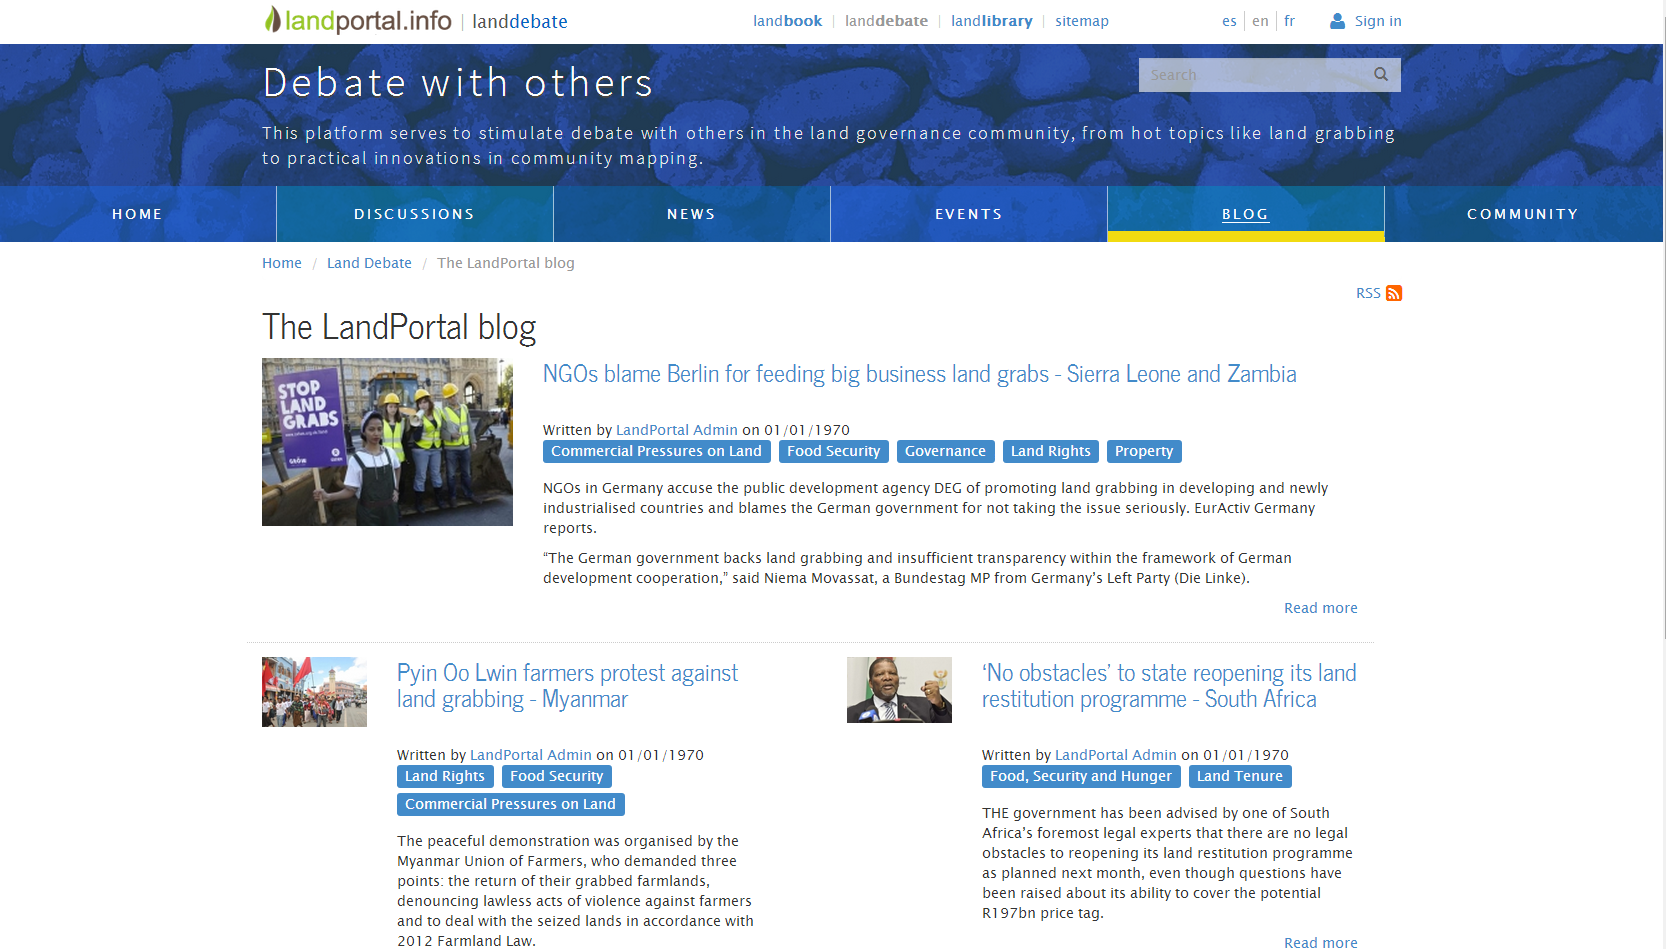
\includegraphics[width=\textwidth]{interfaces/blog}
	\caption{Captura de la vista del blog del Land Portal (inglés)}
	\label{fig:interface_blog}
\end{figure}

\subsection{Vista de detalle de una entrada del blog}
La figura \ref{fig:interface_blog_entry} muestra la interfaz final de una entrada del blog.  Como se puede comprobar no hay muchas variaciones respecto al diseño original, el cual puede observarse en la imagen \ref{fig:mockup_entrada_blog}.

La descripción original de los elementos de esta vista puede consultarse en la sección \ref{chapter04:mockup_blog_entry} perteneciente al capítulo \ref{chapter04}.

\begin{figure}[h]
	\centering
	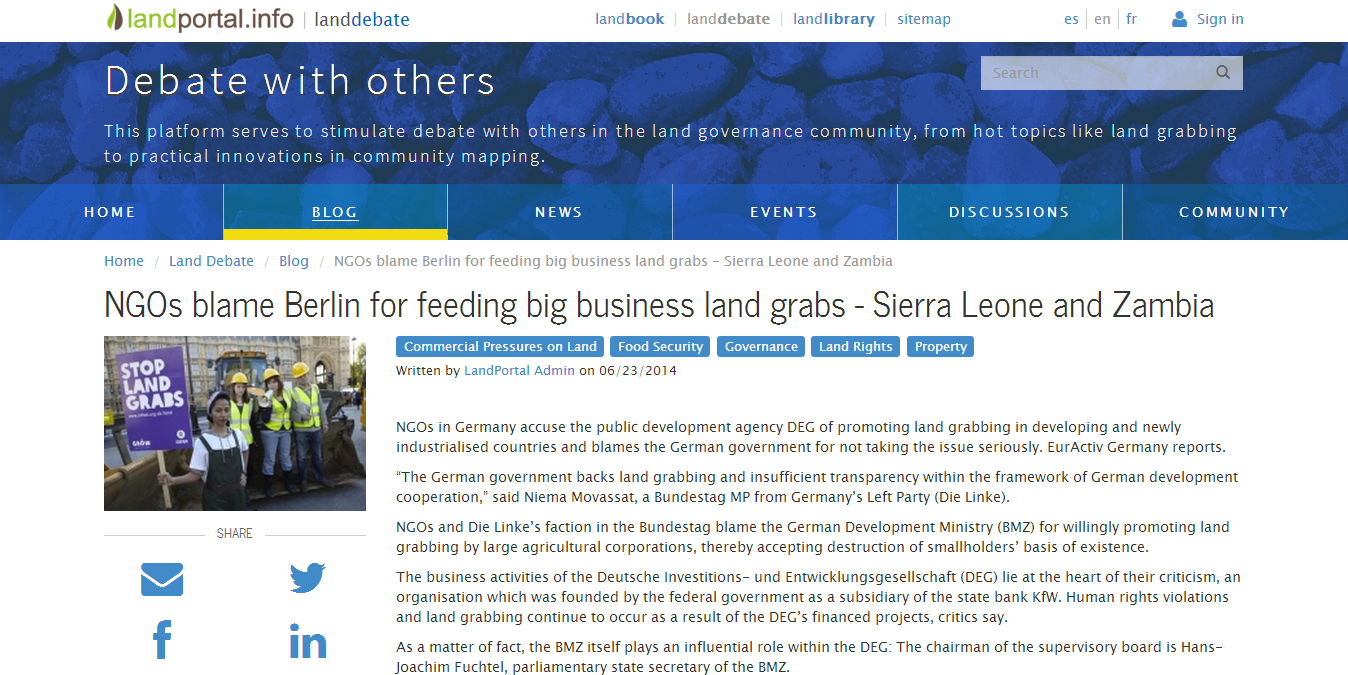
\includegraphics[width=\textwidth]{interfaces/blog-entry}
	\caption{Captura de la vista de detalle de una entrada del blog (inglés)}
	\label{fig:interface_blog_entry}
\end{figure}

\subsection{Vista de eventos}
La figura \ref{fig:interface_eventos} muestra la interfaz final de la vista de eventos.  Como se puede comprobar no hay muchas variaciones respecto al diseño original, el cual puede observarse en la imagen \ref{fig:mockup_eventos}.

La descripción original de los elementos de esta vista puede consultarse en la sección \ref{chapter04:mockup_eventos} perteneciente al capítulo \ref{chapter04}.

\begin{figure}[h]
	\centering
	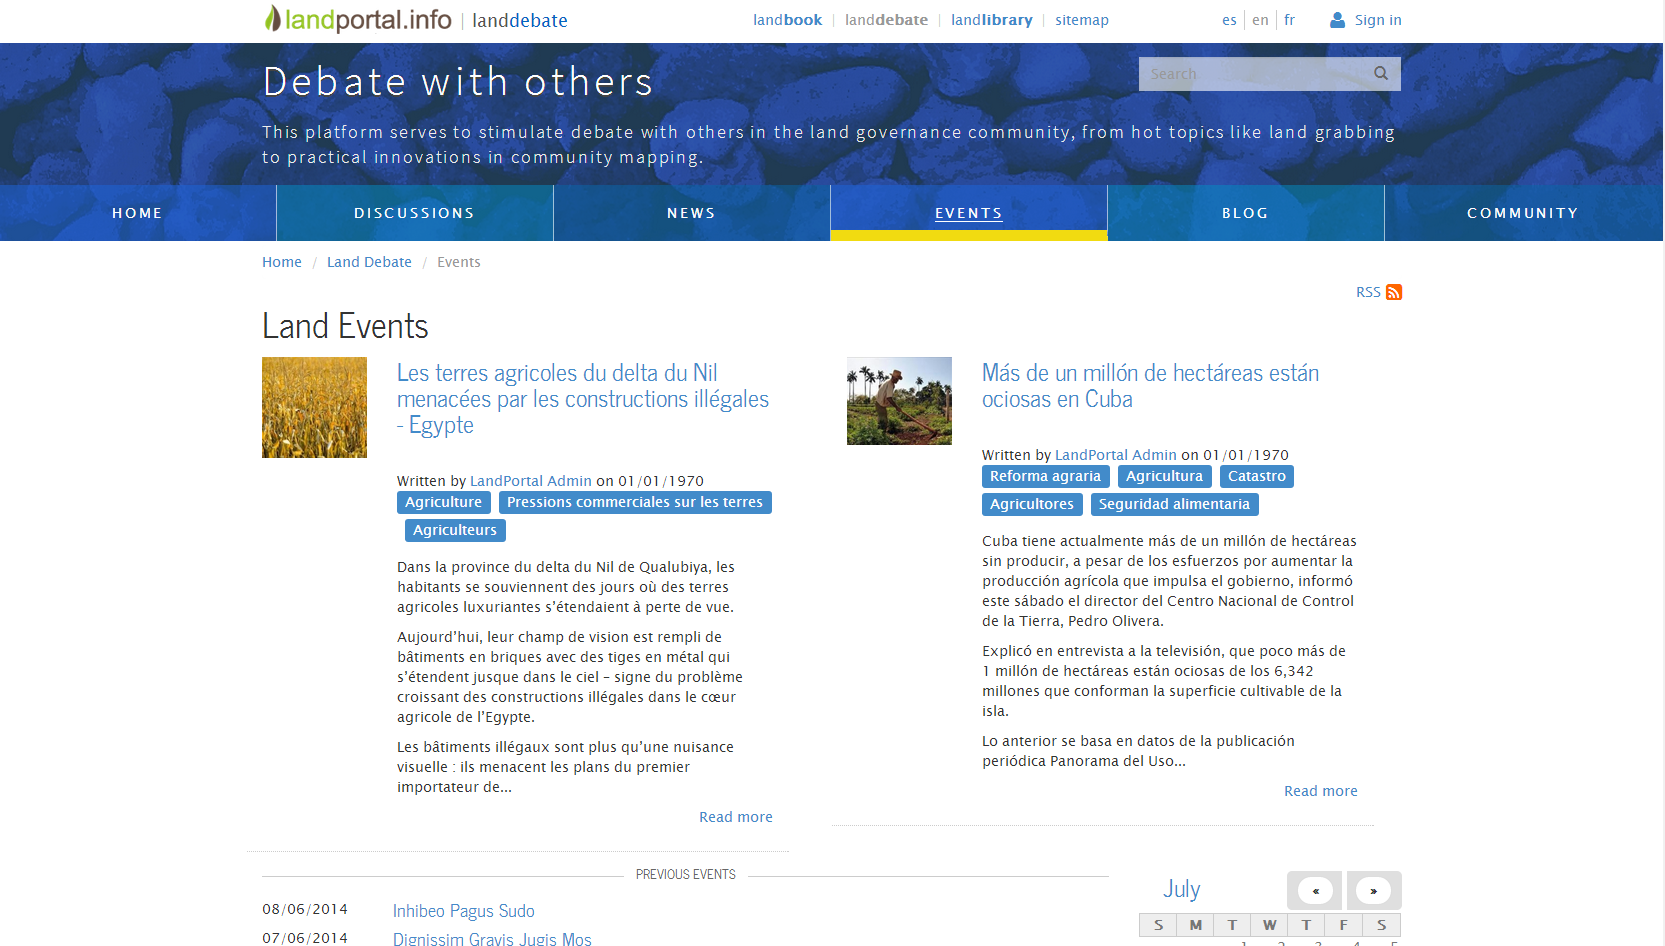
\includegraphics[width=\textwidth]{interfaces/events}
	\caption{Captura de la vista de eventos (inglés)}
	\label{fig:interface_eventos}
\end{figure}


\subsection{Vista de noticias}
La interfaz final de la vista de noticias puede verse en la figura \ref{fig:interface_noticias}, el diseño original para esta vista puede observarse en la imagen \ref{fig:mockup_noticias}.  La descripción original de los elementos de esta vista fue realizada anteriormente en la sección  \ref{chapter04:mockup_noticias} perteneciente al capítulo \ref{chapter04}.

\begin{figure}[h]
	\centering
	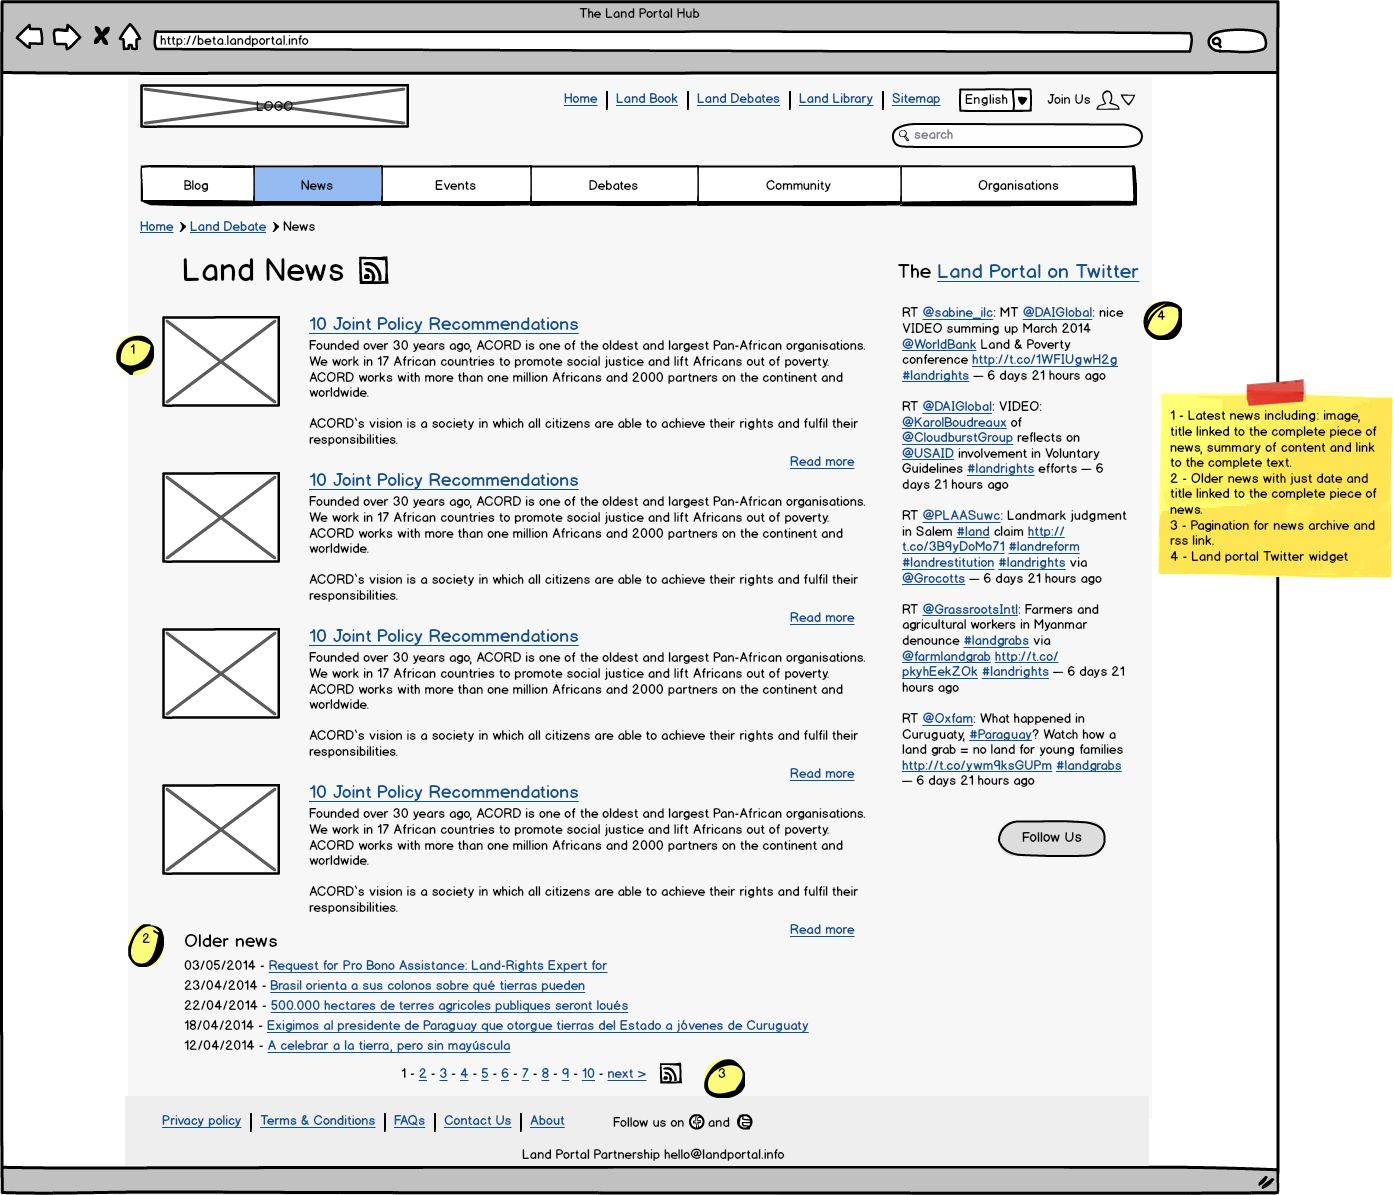
\includegraphics[width=\textwidth]{interfaces/news}
	\caption{Captura de la vista de noticas (inglés)}
	\label{fig:interface_noticias}
\end{figure}


\subsection{Vista de debates}
La figura \ref{fig:interface_debates} muestra el diseño final de la vista de debates. Al igual que en el mockup original (imagen \ref{fig:mockup_debates}), los debates más recientes se muestran de forma destacada y los últimos comentarios se muestran ordenados de más a menos recientes.

Como se puede comprobar, el autor de cada debate se muestra junto a su imagen de perfil.
\begin{figure}[h]
	\centering
	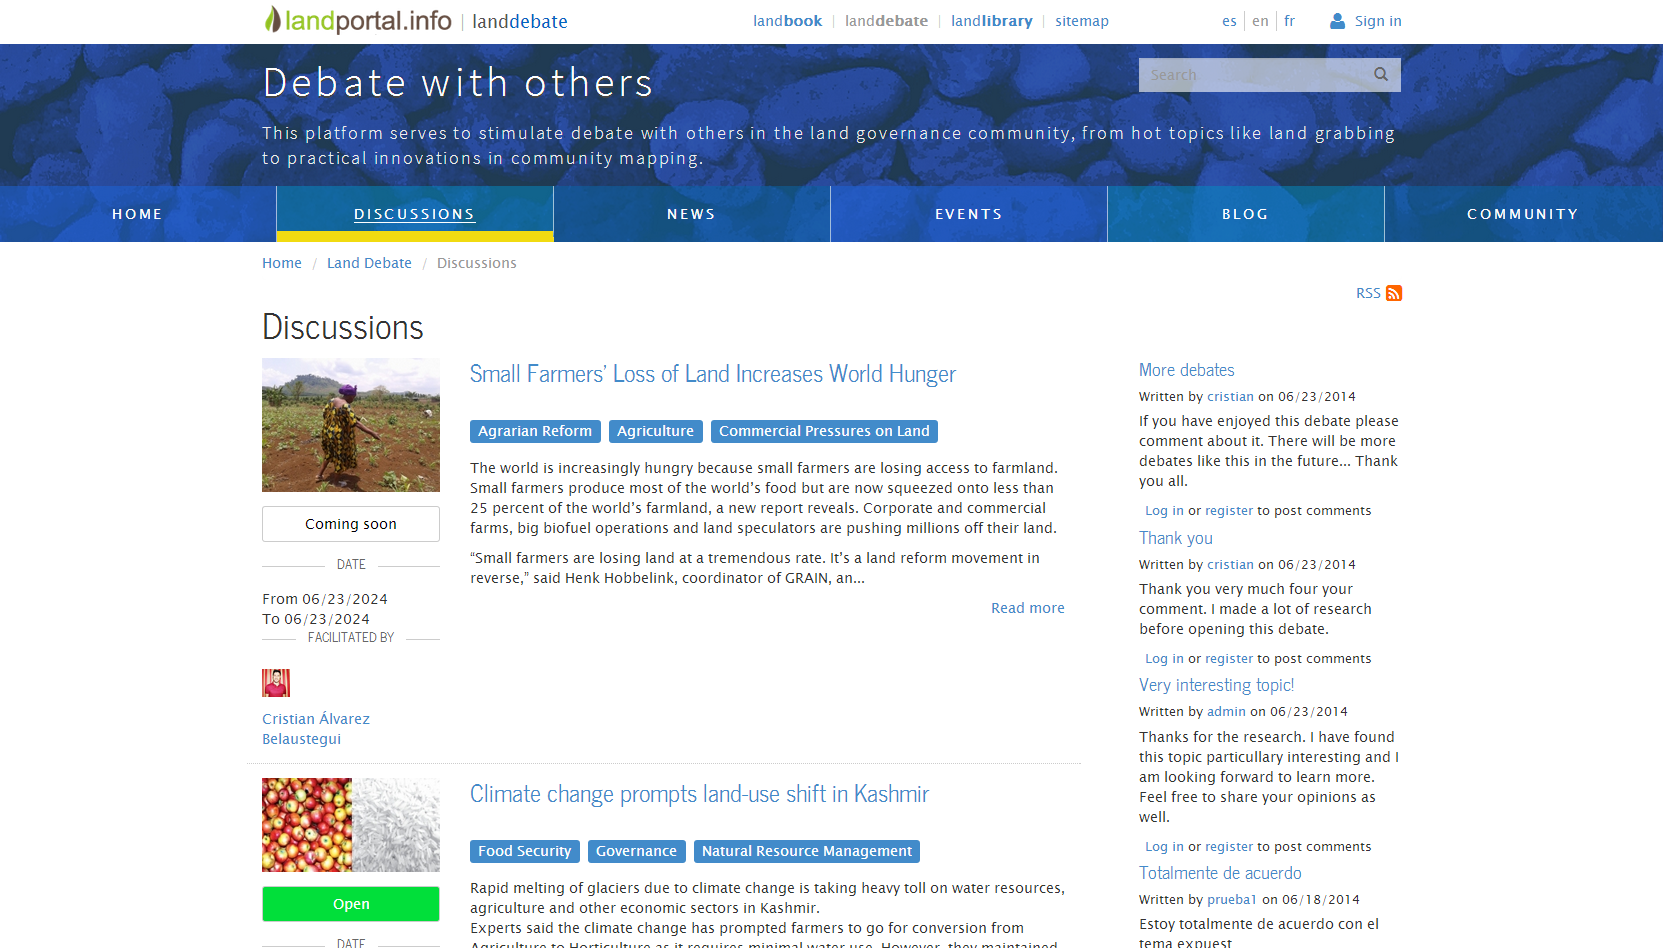
\includegraphics[width=\textwidth]{interfaces/debates}
	\caption{Captura de la vista de debates (inglés)}
	\label{fig:interface_debates}
\end{figure}


\subsection{Vista de detalle de un debate}
La figura \ref{fig:interface_debate} muestra el diseño final de la vista de detalle de un debate,  como se puede observar en la figura \ref{fig:mockup_debate} a penas ha habido variaciones respecto al mockup original.  En la imagen puede verse que el debate está abierto y permite nuevos comentarios de los usuarios así como respuestas a comentarios ya existentes.

\begin{figure}[h]
	\centering
	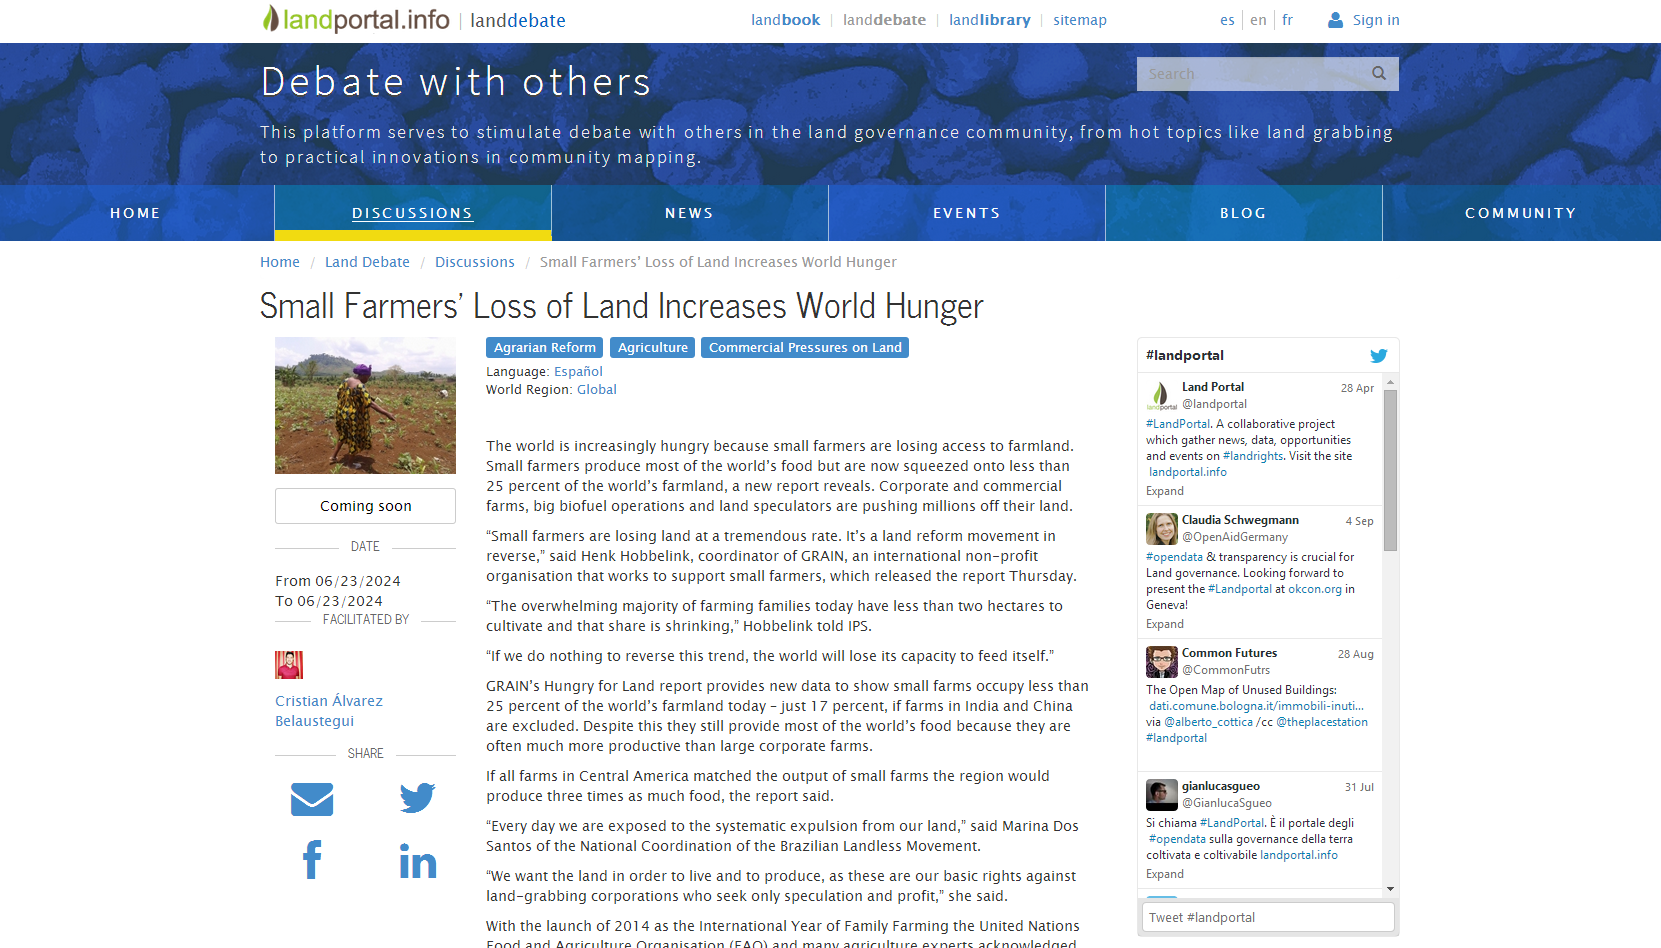
\includegraphics[width=\textwidth]{interfaces/debate}
	\caption{Captura de la vista de detalle de un debate (inglés)}
	\label{fig:interface_debate}
\end{figure}


\subsection{Vista de detalle de una noticia y evento}
En la sección \ref{mockup_noticia_evento} perteneciente al capítulo \ref{chapter04} se explicó que la vista de detalle de una noticia y un evento sería similar a la vista de una entrada del blog (figura \ref{fig:interface_blog_entry}).  La única diferencia sería que las vistas de una noticia o un evento no tendrían sección de comentarios.

Las figuras \ref{fig:interface_noticia} y \ref{fig:interface_evento} muestran respectivamente las vistas de detalle de una noticia y un evento.  Como se puede ver guardan una gran similitud entre sí y respecto al mockup original. 
\begin{figure}[h]
	\centering
	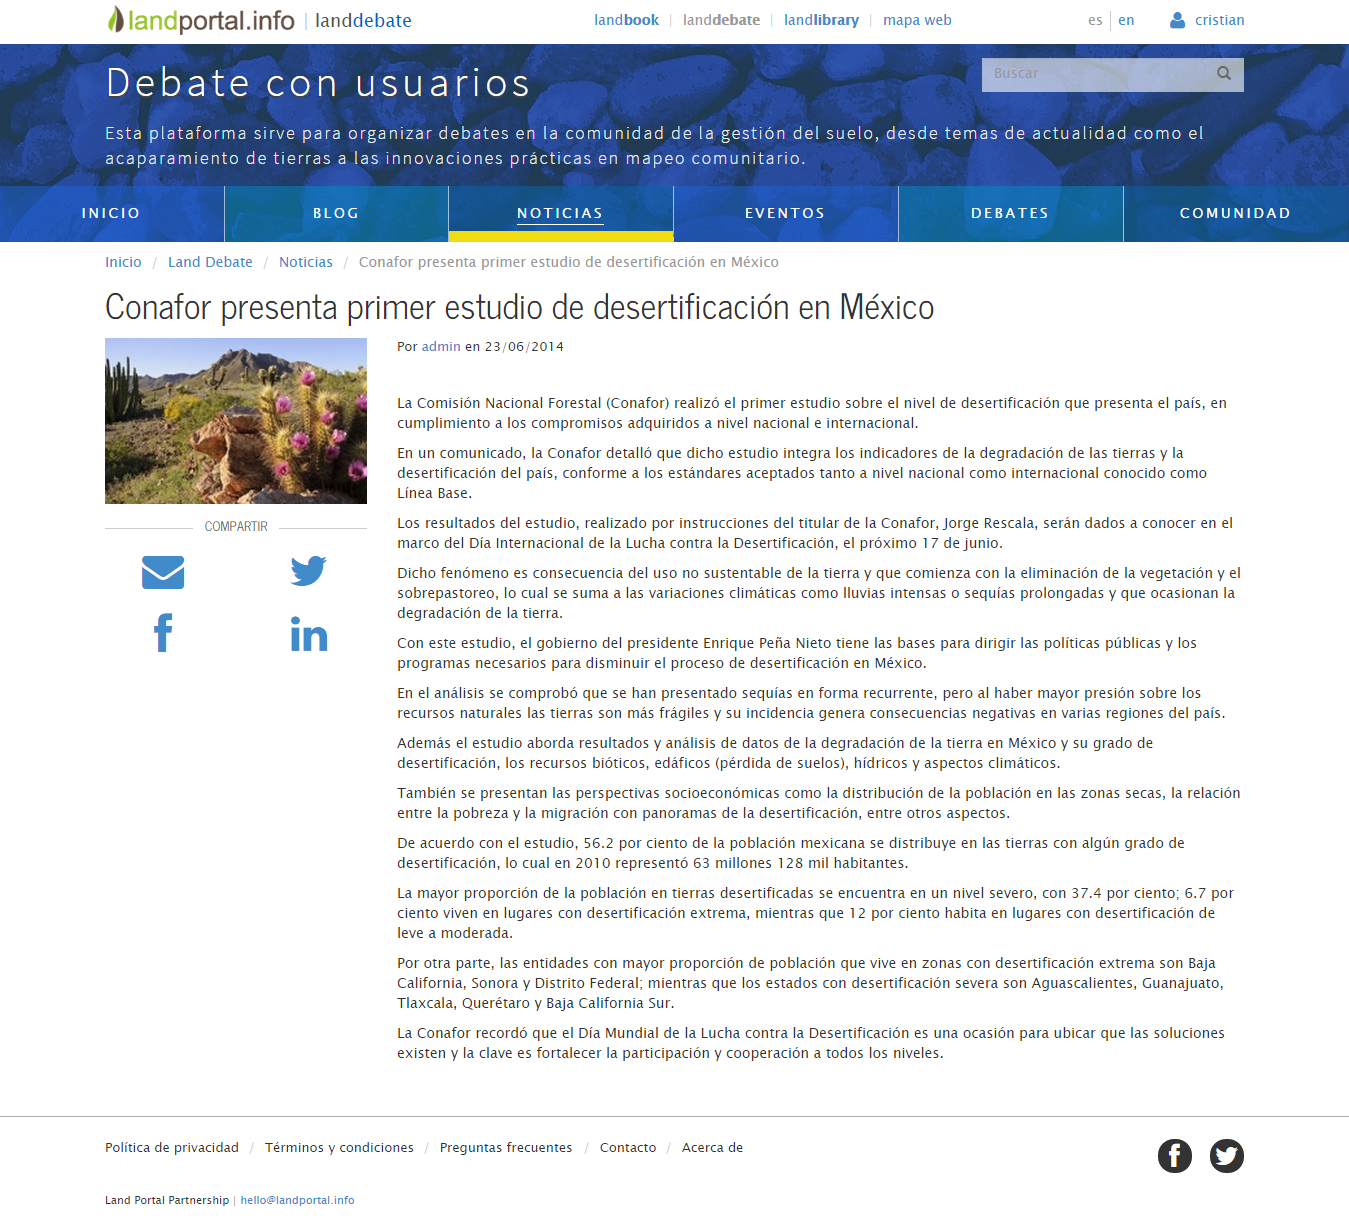
\includegraphics[width=\textwidth]{interfaces/news-entry}
	\caption{Captura de la vista de detalle de una noticia (francés)}
	\label{fig:interface_noticia}
\end{figure}
\begin{figure}[h]
	\centering
	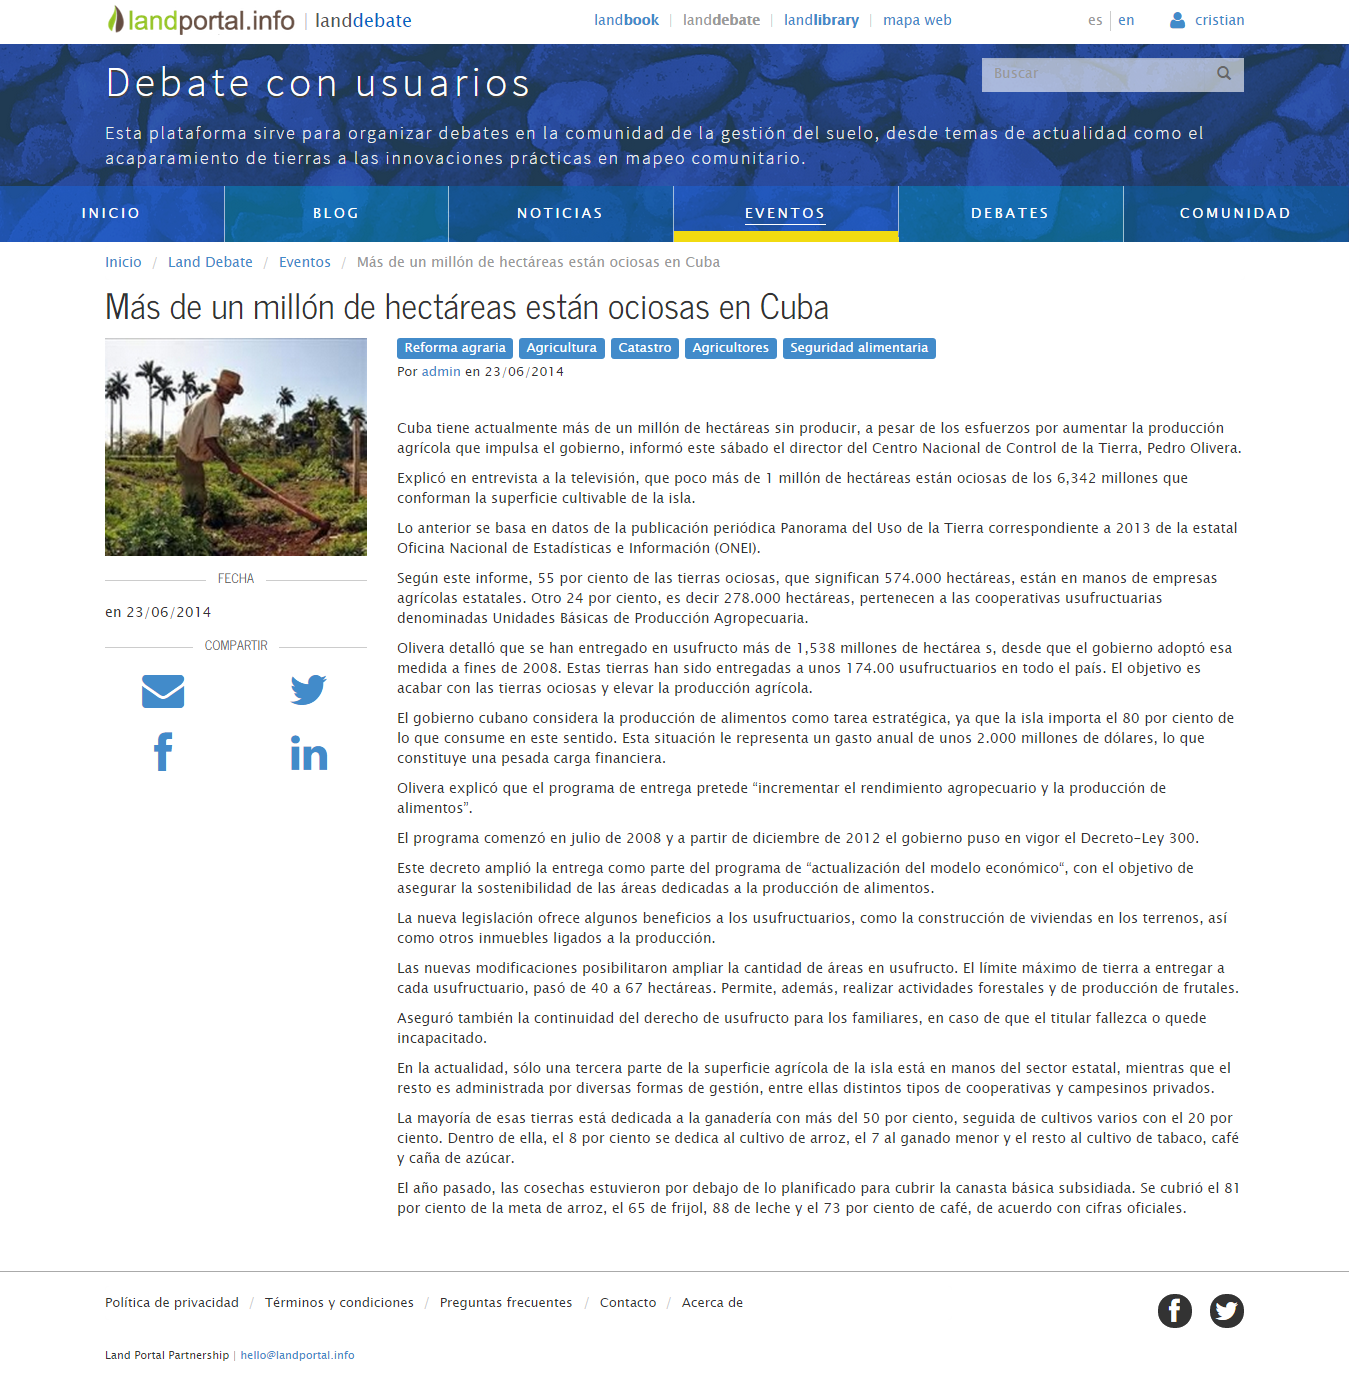
\includegraphics[width=\textwidth]{interfaces/events-entry}
	\caption{Captura de la vista de detalle de un evento (inglés)}
	\label{fig:interface_evento}
\end{figure}


\subsection{Vista de organizaciones}
La figura \ref{fig:interface_organizaciones} muestra el diseño final de la vista de organizaciones.  Al igual que el mockup original (ver la figura \ref{fig:mockup_organizaciones}), esta vista incluye unos controles que permiten la búsqueda de organizaciones por nombre, tópicos relacionados, regiones de operación o países en los que trabajan.  También se incluye un widget de la red social Facebook, para permitir a los usuarios entrar a formar parte de la comunidad de LandPortal en dicha red social.
\begin{figure}[h]
	\centering
	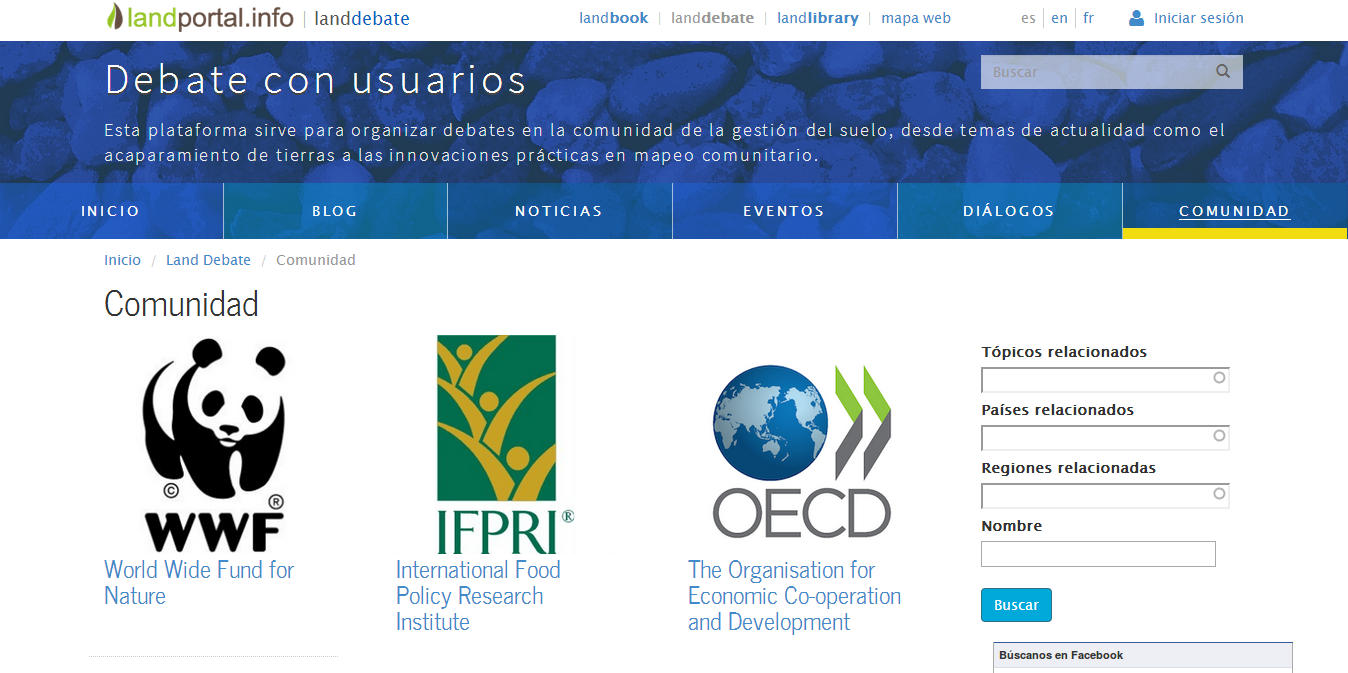
\includegraphics[width=\textwidth]{interfaces/organizations}
	\caption{Captura de la vista de organizaciones (español)}
	\label{fig:interface_organizaciones}
\end{figure}


\subsection{Vista de detalle de una organización}
La figura \ref{fig:interface_organizacion} muestra el diseño final de la vista de organizaciones.  Esta vista no ha sufrido variaciones respecto a su mockup original, dicho mockup puede verse en la figura \ref{fig:mockup_organizacion}.
\begin{figure}[h]
	\centering
	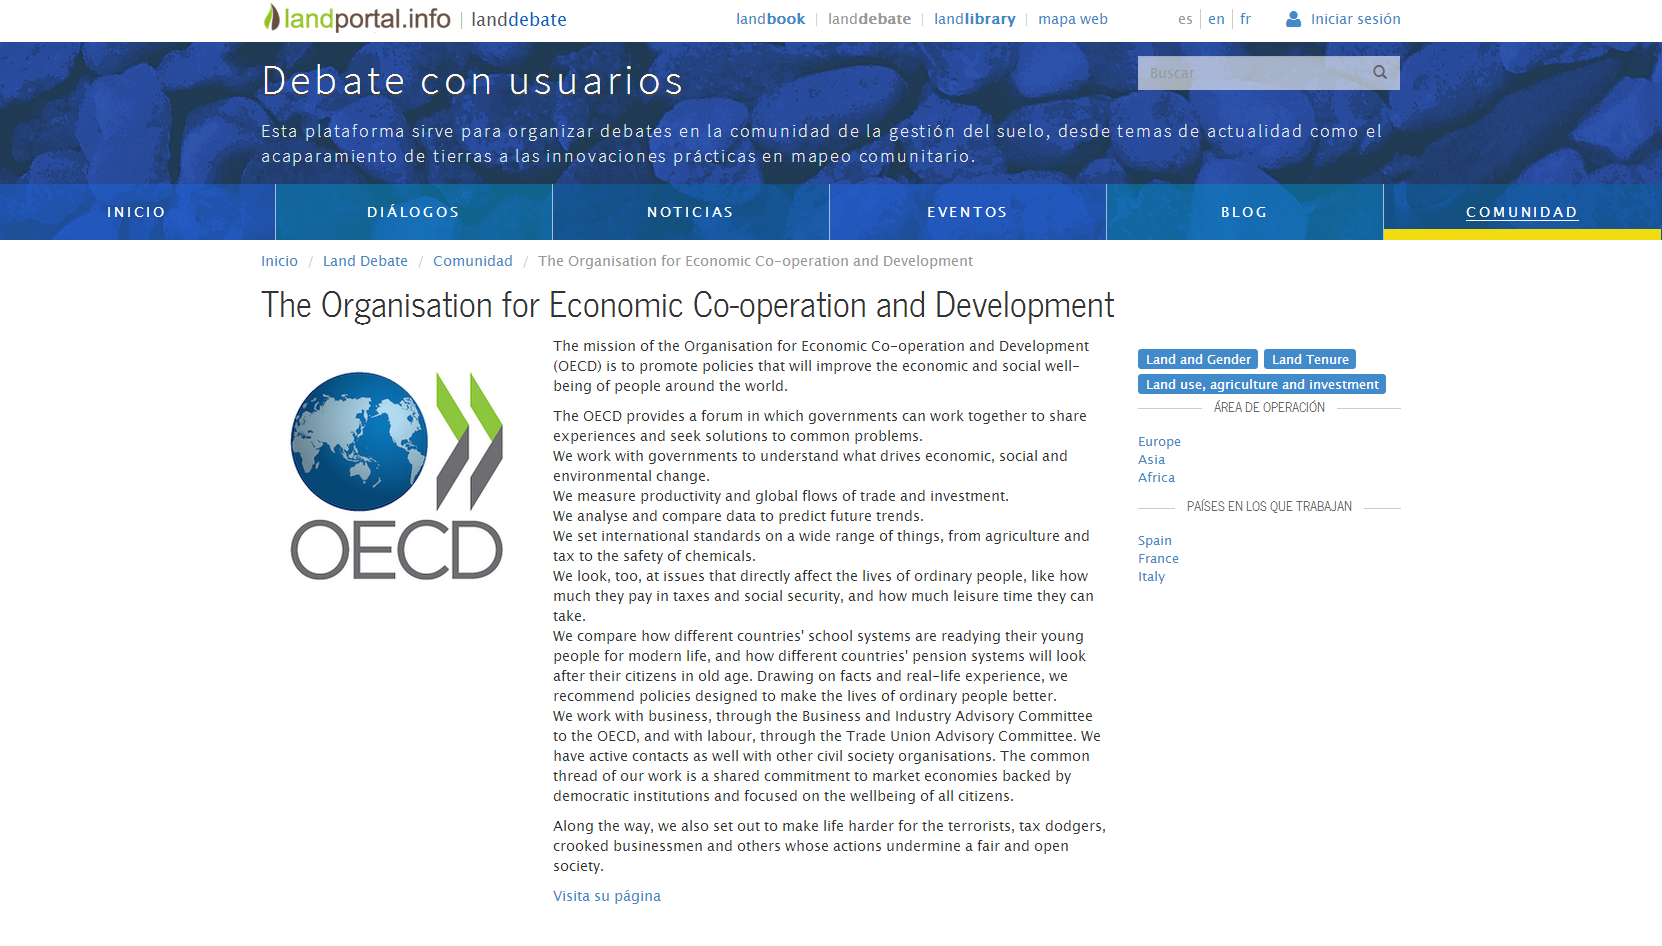
\includegraphics[width=\textwidth]{interfaces/organization}
	\caption{Captura de la vista de detalle de una organización (español)}
	\label{fig:interface_organizacion}
\end{figure}


\subsection{Vista de login}
La interfaz final de la vista de login puede verse en la figura \ref{fig:interface_login},  el mockup original de esta vista puede observarse en la figura \ref{fig:mockup_login}.  

El diseño final sigue las líneas generales del mockup, pero se han añadido unos \textit{placeholders}\footnote{Un \textit{placeholder} es una pequeña guía que describe lo que se espera recibir en un campo de entrada y desaparece cuando el usuario empieza a escribir en él.} a los campos de texto para facilitar la comprensión del usuario.
\begin{figure}[h]
	\centering
	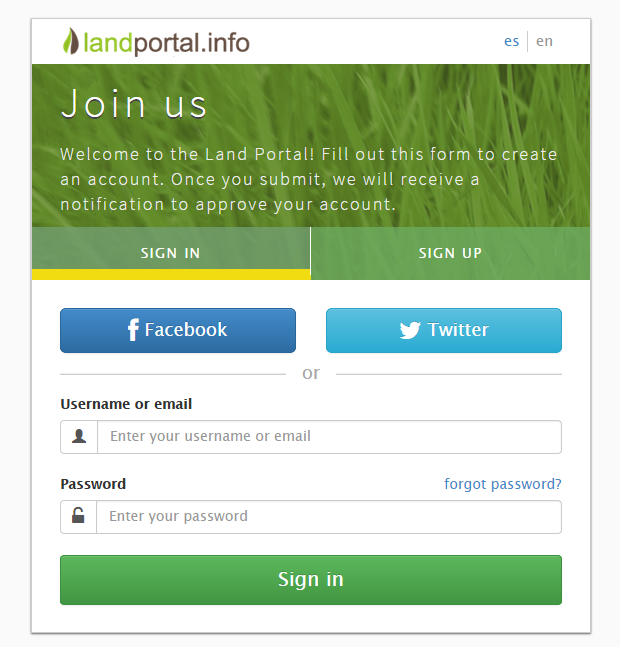
\includegraphics[width=10cm]{interfaces/login}
	\caption{Captura de la vista de login (inglés)}
	\label{fig:interface_login}
\end{figure}


\subsection{Vista de registro}
La figura \ref{fig:interface_registro} muestra el diseño final de la vista de registro en el sistema,  como se puede observar, esta imagen se ha incluido en idioma español.  El mockup original de esta vista puede observarse en la figura \ref{fig:mockup_registro}.

Para aumentar la usabilidad de esta vista, se han incluido unas pequeñas descripciones explicando las reglas para los campos de nombre de usuario y correo electrónico.  Los campos para introducir las regiones y países relacionados cuentan también con un sistema de autocompletado utilizando llamdas AJAX.  Por último, los campos requeridos se han marcado con un asterisco de color rojo con objetivo de hacer más fácil su identificación.
\begin{figure}[h]
	\centering
	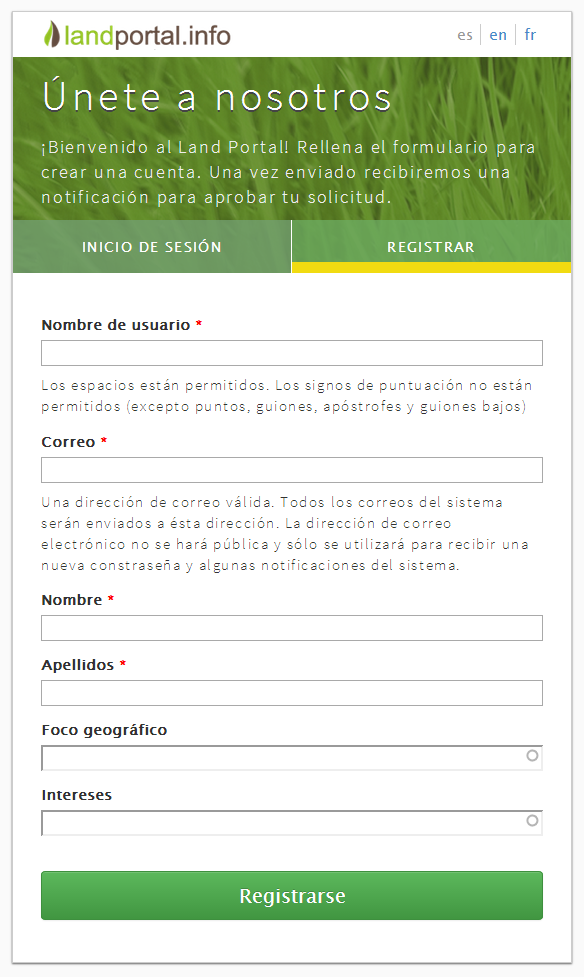
\includegraphics[width=10cm]{interfaces/register}
	\caption{Captura de la vista de registro (español)}
	\label{fig:interface_registro}
\end{figure}


\subsection{Vista del perfil de un usuario}
La figura \ref{fig:interface_perfil_usuario} muestra la vista del perfil de un usuario.  Puesto que esta vista no figuraba entre los mockups de la sección ``\nameref{analisis_interfaces_usuario}'' se describirán aquí sus características:
\begin{itemize}
	\item El nombre de usuario se muestra de forma destacada como título de la vista
	\item El resto de información del usuario se muestra a continuación, con un tamaño más pequeño.  Entre los campos de usuario merece la pena destacar el correo electrónico y la clave de acceso al API.
	\begin{itemize}
		\item Para facilitar el proceso de contactar con el usuario el correo electrónico se incluye como un enlace
		\item La clave de acceso al API sólo se mostrará en aquellos usuarios que tengan permisos de acceso al API.  En cualquier caso, dicha clave no se mostrará al resto de usuarios que visiten el perfil
	\end{itemize}
	\item Los países y regiones en los que el usuario esté interesado también se mostrarán como enlaces, permitiendo cada uno de ellos acceder al resto de elementos del portal etiquetados con el mismo término
	\item Cuando un usuario visite su propio perfil, se incluye un botón que permite editar la información del perfil.  Este botón no se mostrará al resto de usuarios.
\end{itemize}
\begin{figure}[h]
	\centering
	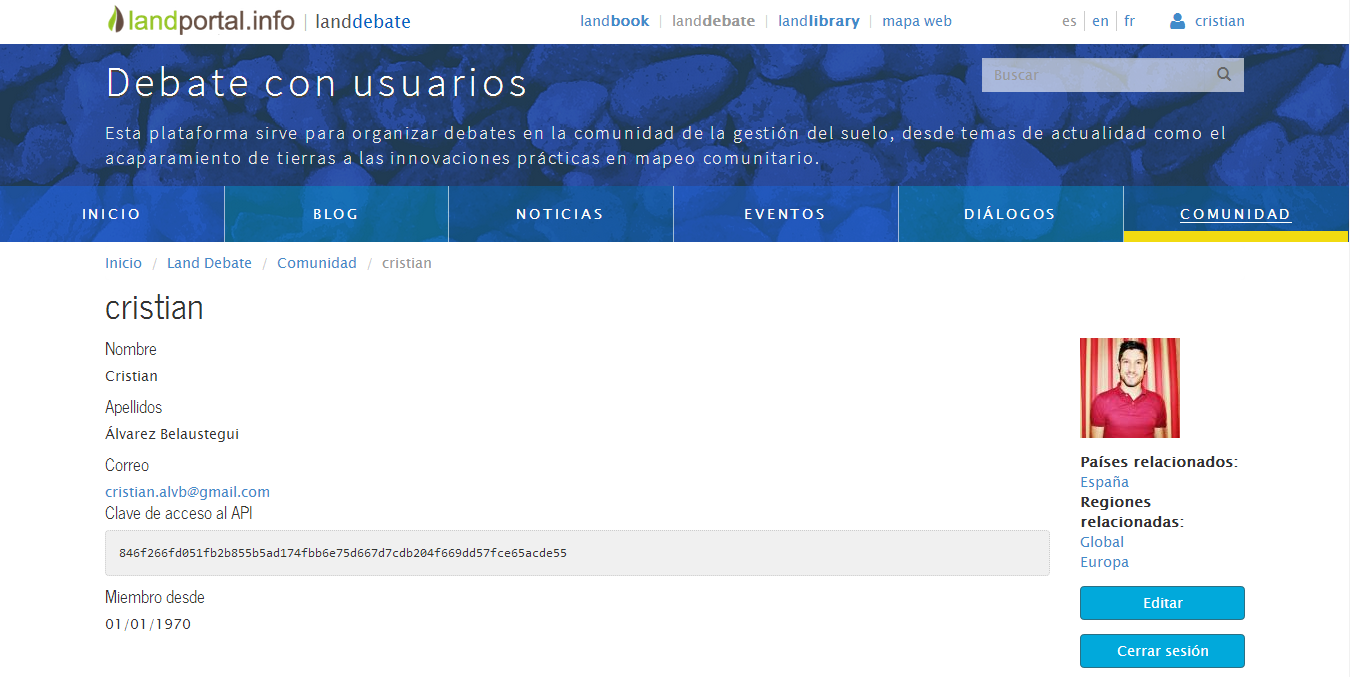
\includegraphics[width=\textwidth]{interfaces/user-profile}
	\caption{Captura de la vista del perfil de un usuario (español)}
	\label{fig:interface_perfil_usuario}
\end{figure}


\subsection{Vista de búsqueda}
La figura \ref{fig:interface_busqued} muestra el diseño final de la vista de búsqueda.  El mockup original de esta vista puede observarse en la figura \ref{fig:mockup_buscar}.

Un pequeño detalle que se ha incluido en esta vista han sido las etiquetas de colores para facilitar a los usuarios la distinción de los tipos de contenido de los resultados.
\begin{figure}[h]
	\centering
	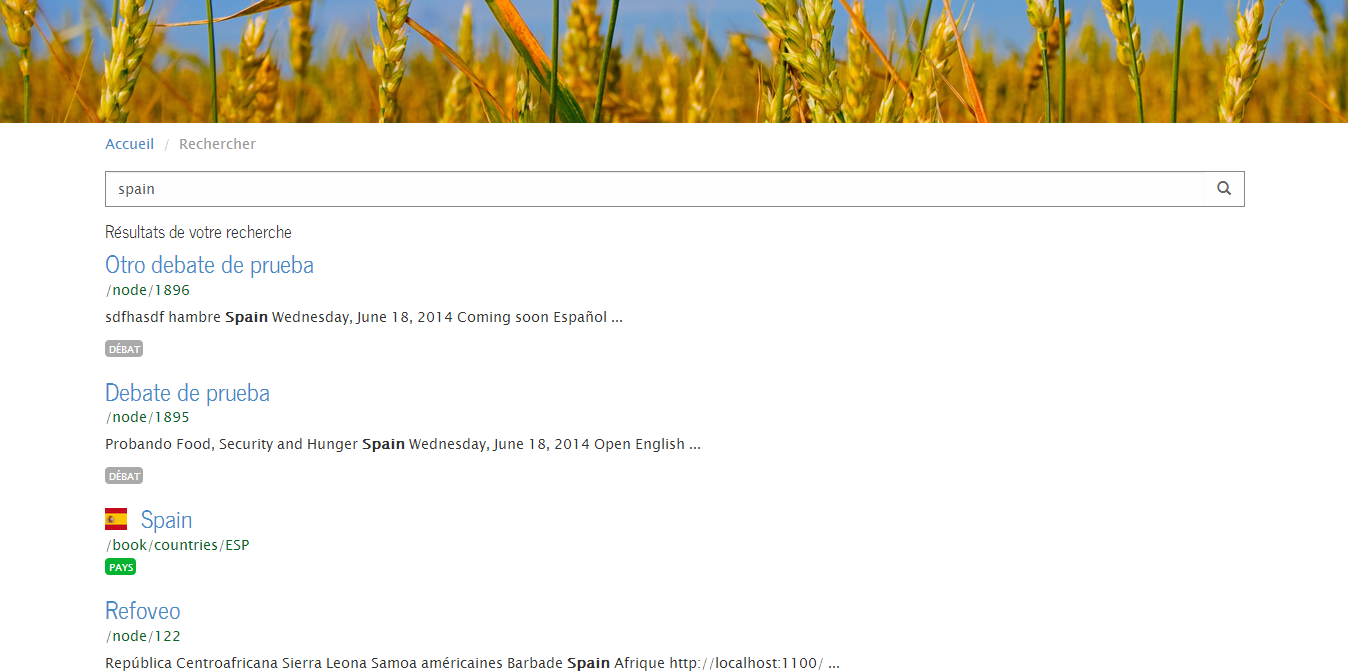
\includegraphics[width=\textwidth]{interfaces/search}
	\caption{Captura de la vista de búsqueda (francés)}
	\label{fig:interface_busqued}
\end{figure}


\subsection{Diseño adaptable}
La interfaz del nuevo Land Portal cuenta con un diseño adaptable o \textit{responsive} con el fin de que pueda mostrarse correctamente aprovechando el espacio ofrecido por los distintos dispositivos como \textit{smartphones} o \textit{tablets}.

La figura \ref{fig:interface_responsive} muestra la interfaz de la vista del blog en un tamaño de pantalla pequeño y la interfaz de la vista de los debates en un tamaño de pantalla intermedio.

\begin{figure}[h]
	\centering
	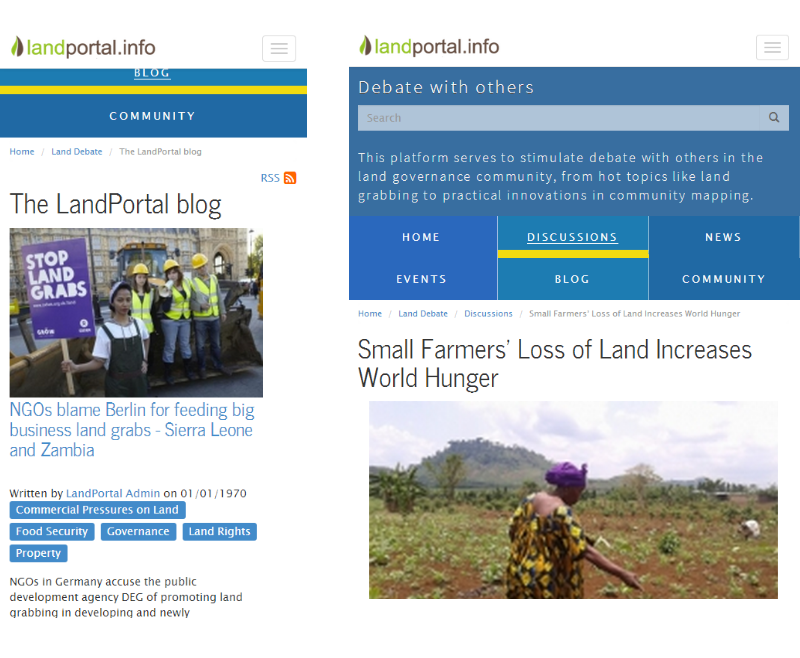
\includegraphics[width=\textwidth]{interfaces/responsive}
	\caption{Captura del diseño adaptable (inglés)}
	\label{fig:interface_responsive}
\end{figure}